
% rubber: module pdftex
\documentclass[english,aspectratio=43,8pt]{beamer}
\usepackage{graphicx}
\usepackage{amssymb}
\usepackage{booktabs}
\usepackage{siunitx}
\usepackage{subcaption}
\usepackage{marvosym}
\usepackage{verbatim}
\usepackage[normalem]{ulem}  % Needed for /sout

\newcommand{\pb}{\si{\pico\barn}}%
\newcommand{\fb}{\si{\femto\barn}}%
\newcommand{\invfb}{\si{\per\femto\barn}}
\newcommand{\GeV}{\si{\giga\electronvolt}}

\hypersetup{colorlinks=true,urlcolor=blue}
\usetheme[]{bjeldbak}


%%% For wider frames
\newcommand\Wider[2][3em]{%
\makebox[\linewidth][c]{%
  \begin{minipage}{\dimexpr\textwidth+#1\relax}
  \raggedright#2
  \end{minipage}%
  }%
}
%%% For wider frames end

\newcommand{\backupbegin}{%
   \newcounter{finalframe}
   \setcounter{finalframe}{\value{framenumber}}
}
\newcommand{\backupend}{%
   \setcounter{framenumber}{\value{finalframe}}
}

\newcommand\blfootnote[1]{%
  \begingroup
  \renewcommand\thefootnote{}\footnote{#1}%
  \addtocounter{footnote}{-1}%
  \endgroup
}

\begin{document}

\title{Gantry setup at FNAL}
\author[C. Fangmeier]{\textbf{Caleb Fangmeier}}
\institute[UNL]{University of Nebraska \-- Lincoln}
\date{ETL Metting | Dec 9, 2019}

\titlegraphic{%
\begin{figure}
  \includegraphics[width=1in]{CMSlogo.png}\hspace{0.75in}\includegraphics[width=1in]{nebraska-n.png}
\end{figure}
}

\begin{frame}[plain]
  \titlepage%
\end{frame}

\begin{frame}{Introduction}
      \begin{itemize}
          \item Aerotech 3+1 axis gantries were used sucessfully in Phase I FPIX at Nebraska and Purdue
          \item Nebraska, Purdue, and CUA will be using such gantries again for Phase II TFPX
          \item Such gantries will be used for ETL module assembly
          \item ETL assembly sites:
            \begin{itemize}
                \item Nebraska - Gantry ordered, expected delivery roughly May
                \item SiDet @ FNAL - Existing gantry recomissioned
            \end{itemize}
      \end{itemize}
\end{frame}

\begin{frame}{Gantry System Overview}
    \begin{figure}
        \includegraphics[width=\textwidth]{figures/gantry.png}
    \end{figure}
\end{frame}

\begin{frame}{ETL Module assembly steps}
    \begin{columns}
    \begin{column}{0.5\textwidth}
    \begin{enumerate}
        \item Operator places baseplates and sensor assembly onto chucks
        \item Vision system is used to do position fine-tuning (few micron level)
        \item Gantry grabs a stamp, dips it in glue, and applies the glue to the baseplate
        \item Gantry picks a sensor assembly and places it on the baseplate
        \item Gantry grabs weight and places it on sensor assembly
        \item Repeat 3-5 for other modules
        \item Allow glue to cure (at least partially) before removing modules from gantry table
    \end{enumerate}
    Attaching of cover plate follows similar steps
    \end{column}
    \begin{column}{0.5\textwidth}
        \begin{figure}
            \includegraphics[width=\textwidth]{figures/ETL_module.png}
        \end{figure}
    \end{column}
\end{columns}
\end{frame}

\begin{frame}{Software Automation}
    \begin{itemize}
        \item During Phase I production, control software was developed to automate the process of gluing and encapsulation.
        \item Written observing LabVIEW best practices. Split between ``applications'' and an underlying library.
        \item Library includes
          \begin{itemize}
              \item Access to all hardware (Gantry, vacuum, cameras\ldots)
              \item Fiducial pattern recognition
              \item Calculation of part location from fiducials
              \item Atomic motion operations (Pickup a tool, Move to chuck X, etc)
          \end{itemize}
        \item Existing applications include:
            \begin{itemize}
                \item (Legacy) Gluing Application
                \item (Legacy) Potting Application
                \item gScript Application
            \end{itemize}
    \end{itemize}
\end{frame}

\begin{frame}{gScript Application}
  \begin{columns}
    \begin{column}{0.35\textwidth}
      \begin{itemize}
          \item Implements simple text-based command language called gScript
          \item Developed in Spring 2019 as a replacement for Purdue's legacy scripting tool
          \item Enables quick prototyping of gantry procedures
          \item Example script (right) retrieves a tool from the tool rack and replaces it
          \item \href{https://youtu.be/5qrpeWGLro0}{Script in action!}
          \item All gantry software, including the gScript interpreter, can be found \href{https://github.com/CUASAS/pixel-gantry-control}{here}.
      \end{itemize}
    \end{column}
    \begin{column}{0.65\textwidth}
    \begin{figure}
        \includegraphics[width=\textwidth]{figures/gScript_UI.PNG}
    \end{figure}
  \end{column}
  \end{columns}
\end{frame}


\begin{frame}{Status at FNAL}
    \begin{figure}
        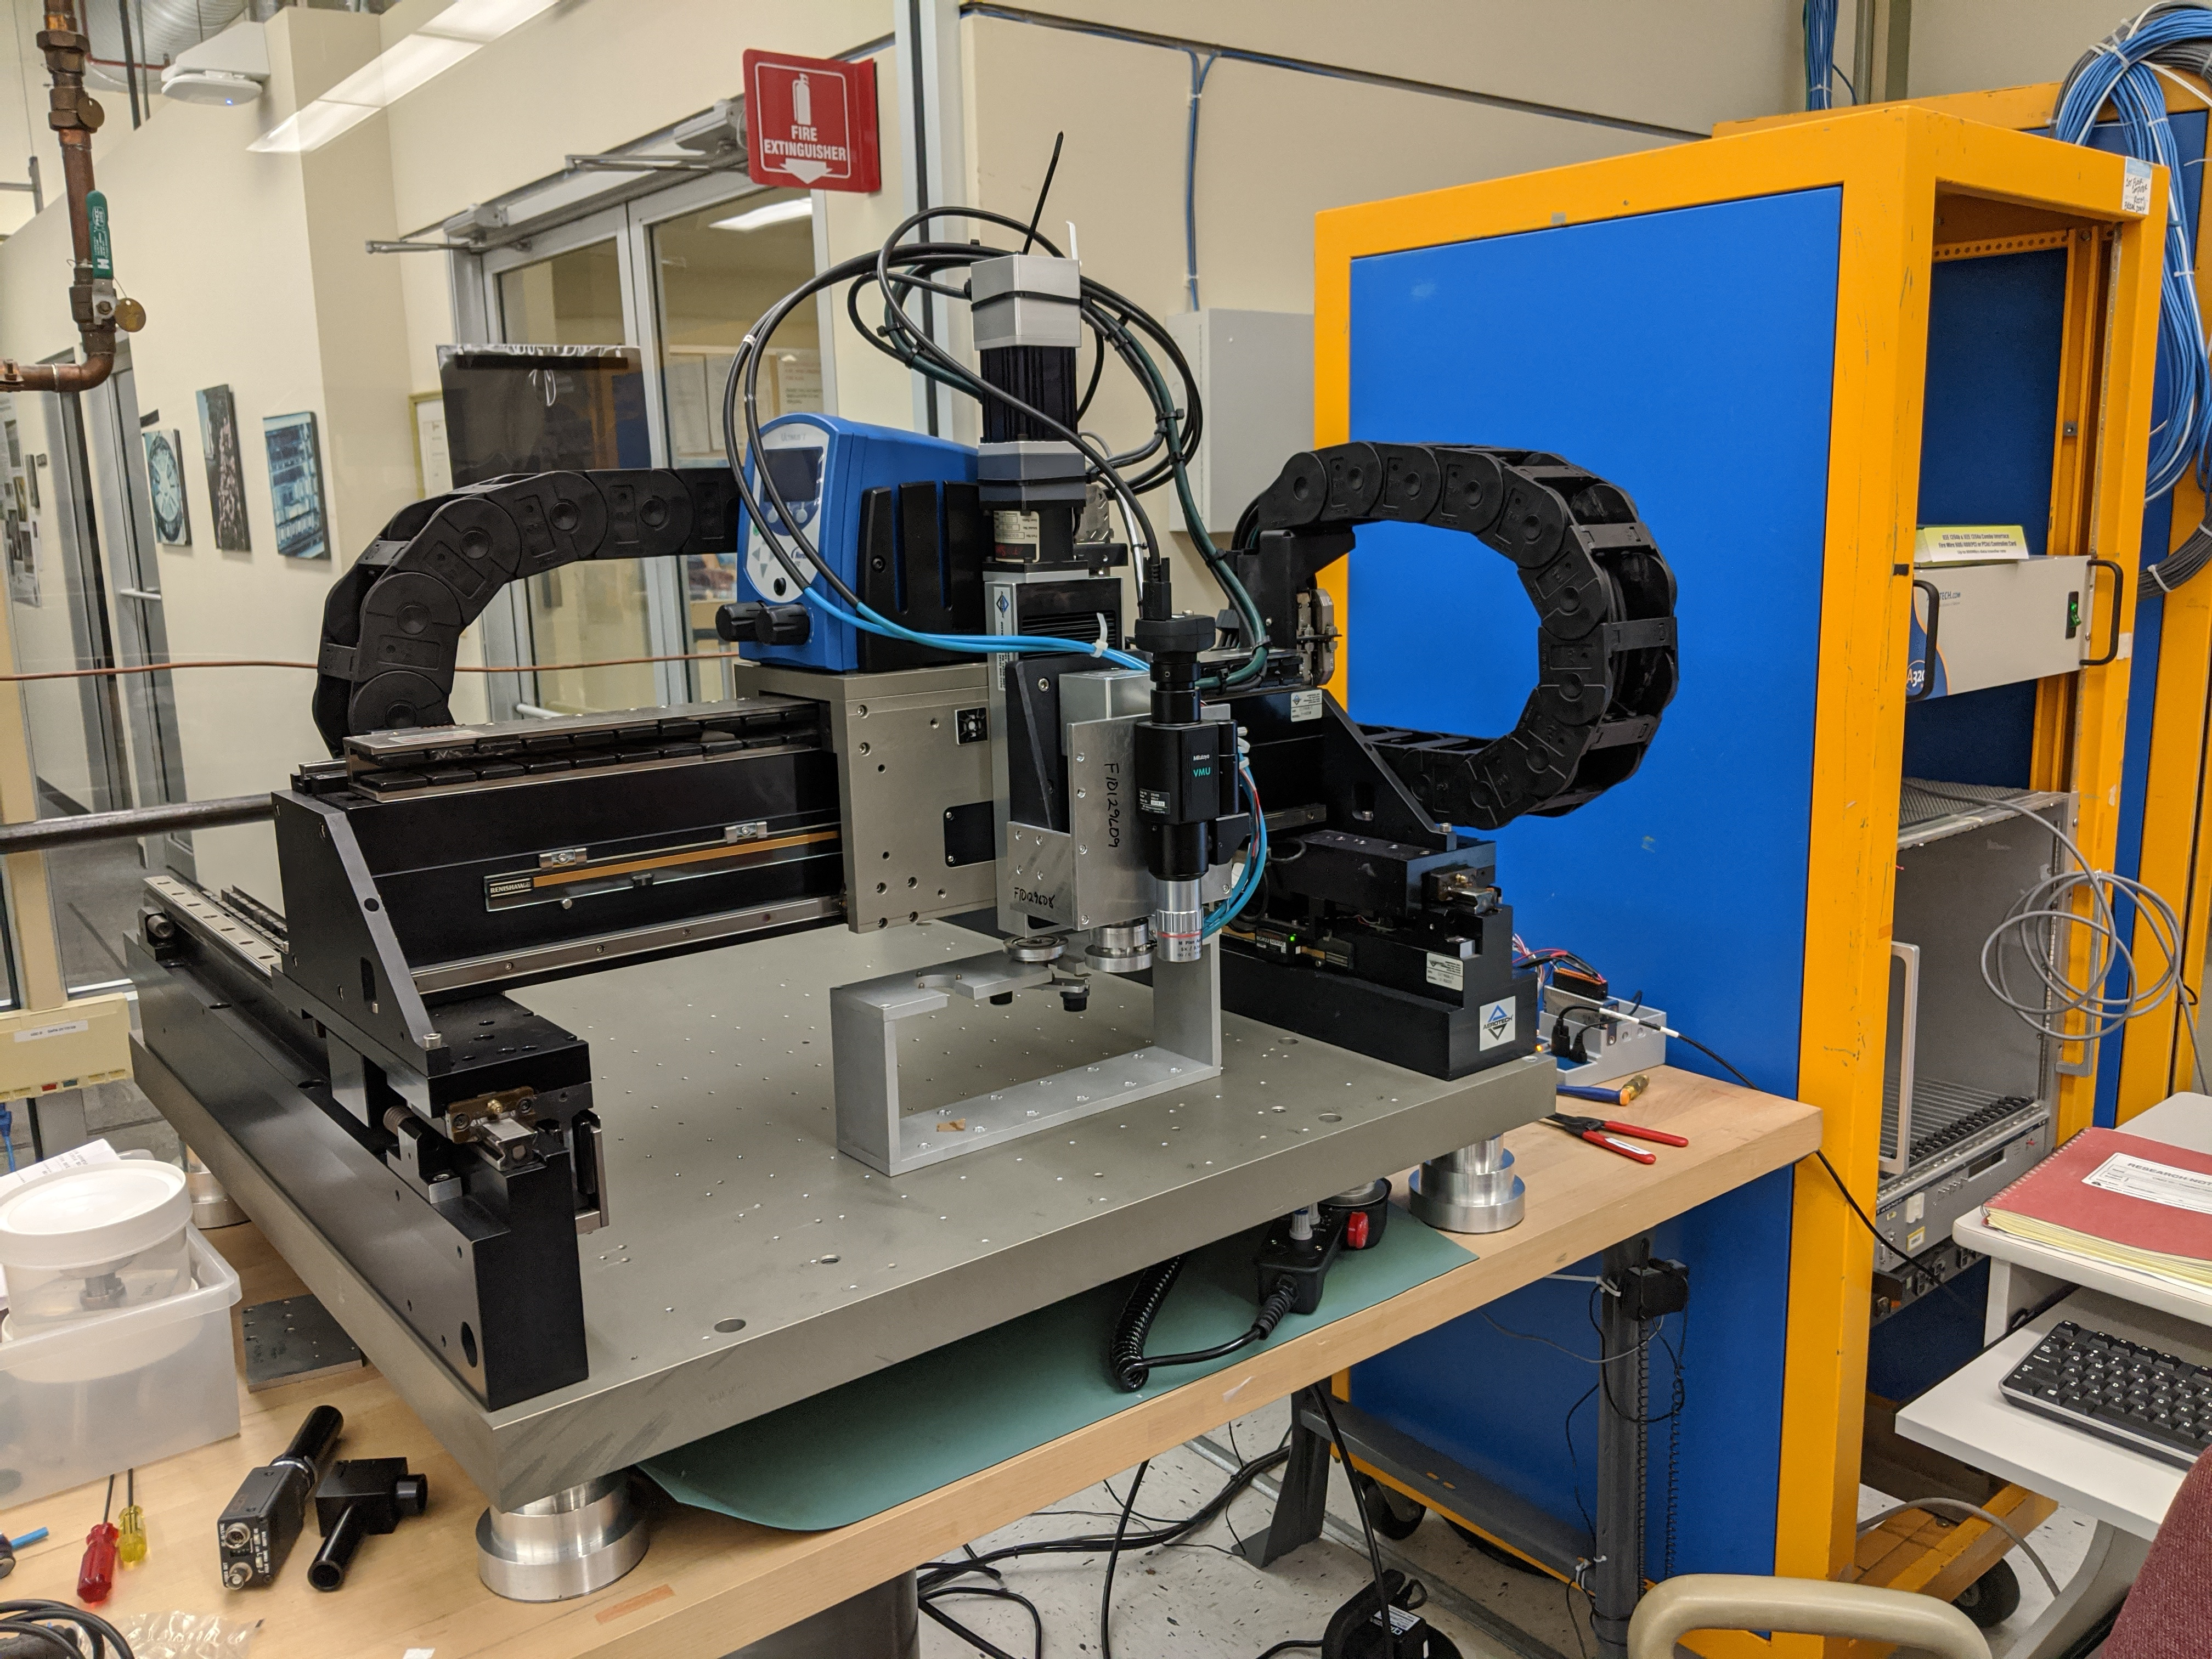
\includegraphics[width=\textwidth]{figures/FNAL_gantry.jpg}
    \end{figure}
\end{frame}

\begin{frame}{Status at FNAL}
  \begin{columns}
    \begin{column}{0.5\textwidth}
      \begin{itemize}
          \item Hardware closely approximating Phase I gantry setup installed including:
            \begin{itemize}
              \item Gantry hand controller
              \item Gantry-head camera with associated optics
              \item Vacuum pump, manifold, and controller
              \item Legacy fixtures (ok for now, will require adjustments at some point)
            \end{itemize}
          \item Software deployed on FNAL Computer and operator given basic training on its use
          \item Custom fixtures for ETL modules under development
          \item Next step is to demonstrate sucessful pick-n-place using dummy parts
      \end{itemize}
    \end{column}
    \begin{column}{0.5\textwidth}
        \begin{figure}
            \includegraphics[width=\textwidth]{figures/isoview_ETLassembly.jpg}
        \end{figure}
        \begin{figure}
            \includegraphics[width=\textwidth]{figures/ETL_single_assychuck2.png}
        \end{figure}
    \end{column}
  \end{columns}
\end{frame}

% \begin{frame}
%     \begin{figure}
%         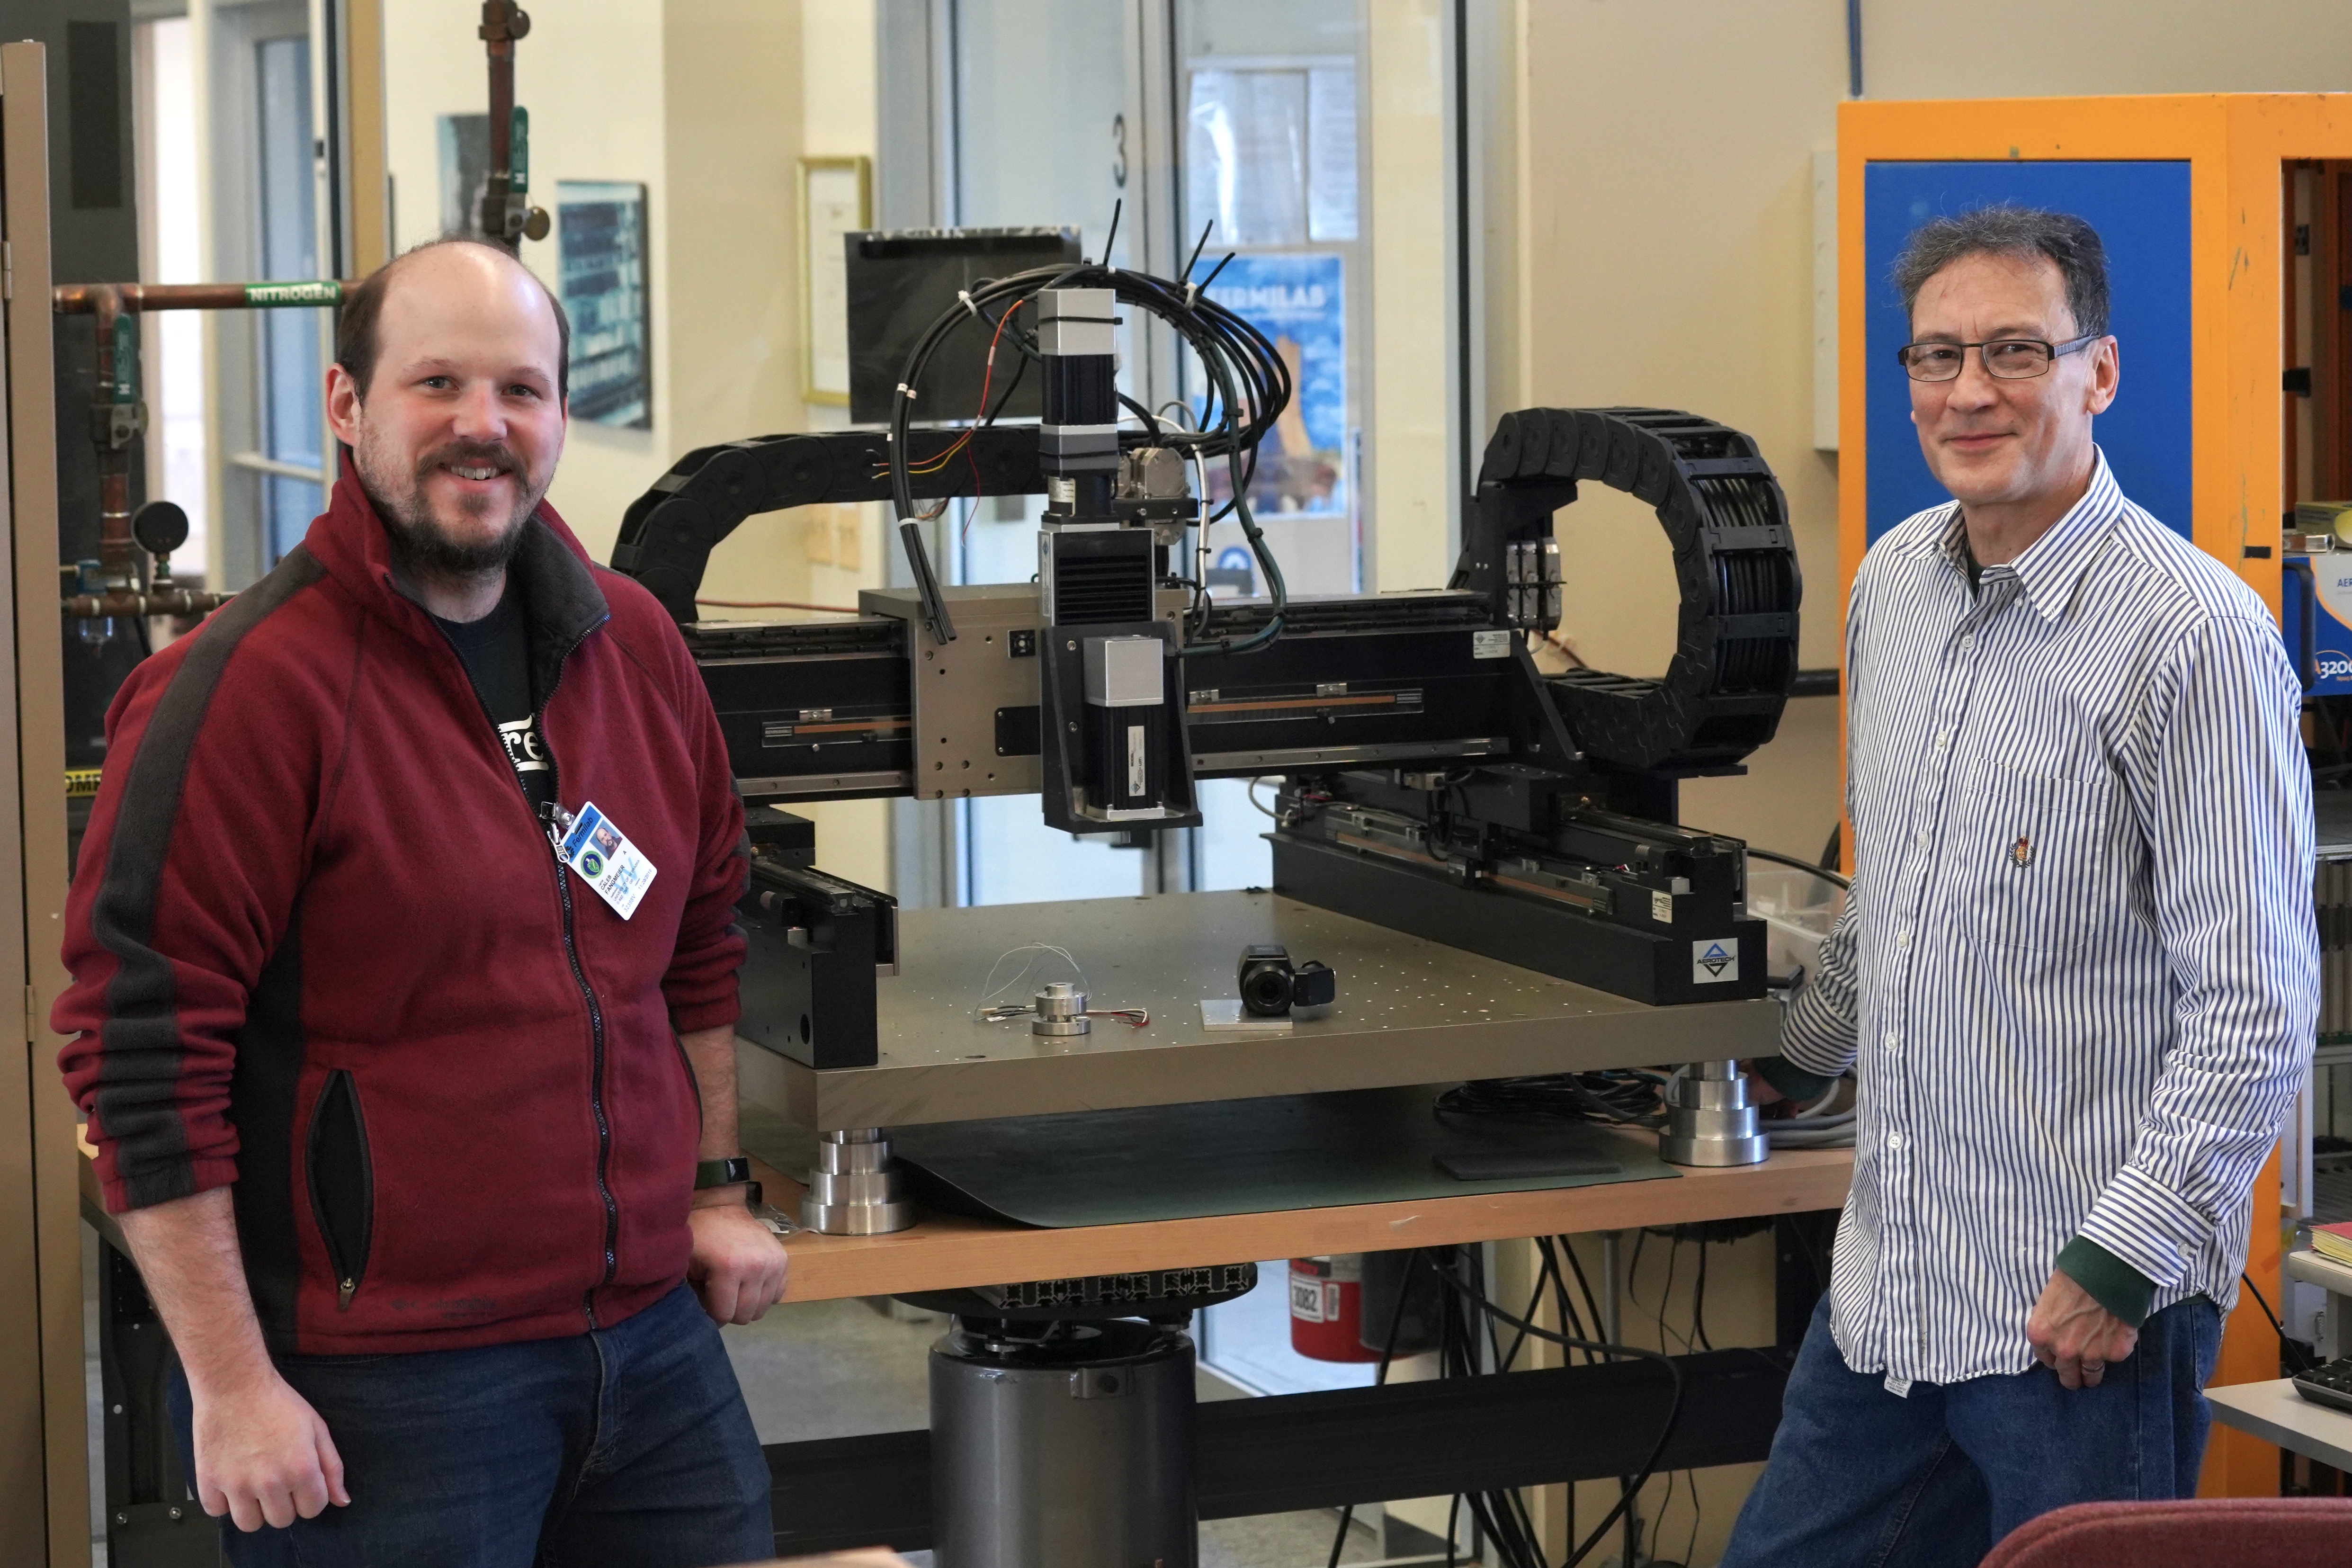
\includegraphics[width=\textwidth]{figures/teamwork.jpg}
%     \end{figure}
% \end{frame}

% \appendix
% \backupbegin%

% \begin{frame}
%   \begin{center}
%     {\Huge BACKUP}
%   \end{center}
% \end{frame}



% \backupend%

\end{document}
